\documentclass[a4paper]{article}
\usepackage[utf8]{inputenc}
\usepackage{fullpage}
\usepackage{csquotes}
\usepackage[ngerman]{babel}
\usepackage{biblatex}
\usepackage{float}
\usepackage{graphicx}
\usepackage{subfigure}
\usepackage{graphvizzz}
\usepackage{hyperref}
\usepackage{minted}
\usemintedstyle{default}
\bibliography{documentation}
\title{PowPow Dokumention}
\author{Willi Schönborn}
\date{\today}
\begin{document}

\begin{figure}[H]
\centering

\includegraphics{beuth.png}
\maketitle
\end{figure}

\newpage
\tableofcontents

\newpage
\section{Einleitung}
Als Teil der Lehrveranstaltung \textit{Computer Graphics and Effects} im Sommersemester 2011 an der \textit{Beuth Hochschule für Technik Berlin} sollte im Rahmen eines Semester-Projektes ein Spiele-Prototyp auf Basis der jVR-Rendering-Engine entstehen. Ziel dieses Dokumentes ist es, die Idee sowie das Produkt dieses Projektes zu beschreiben und erläutern.

\subsection{Idee}
Als Idee für den Prototypen dient das Space-Arcade-Spiel \textit{PewPew} das für die Android-Plattform entwickelt wurde. Markante Eigenschaften des Spiels sind die sehr simpel anmutende Spielgrafik, die einzig und allein auf  einfachste Wireframe-Modelle setzt, sowie eine Verfolgungskamera, die sich ausschließlich in einer Ebene bewegt. Die Steuerung von PewPew erfolgt mithilfe der beiden Daumen auf zwei virtuellen Joysticks in den unteren Ecken des Bildschirms.

\begin{figure}[H]
\centering
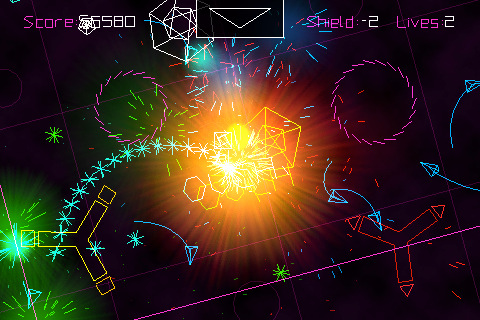
\includegraphics[width=0.7\textwidth]{PewPew-iPhone-App-Review.jpg}
\caption{PewPew In-Game Screenshot}
\end{figure}

Der zu Prototyp sollte einzelne dieser Eigenschaften beinhalten, ohne dabei zu viele Elemente der eigentlichen Spielidee zu übernehmen um den Aufwand in einem überschaubaren Rahmen zu halten. Das Look-and-Feel des Prototypen sollte in etwa dem des Originalspiels entsprechen.

\newpage
\section{Funktionsweise}
Die Steuerung des Spiels unterscheidet zwischen Bewegung und Feuerrichtung. Beide Dinge können unabhängig voneinander bedient werden. Das funktioniert sowohl mit der Tastatur als auch mit einem angeschlossenen Gamepad, wobei die Variante mit einem Gamepad wesentlich flüssiger von der Hand geht. Mit dem linken Analog-Stick steuert man die Bewegung des Raumschiffs und mit dem rechten die Feuerrichtung. 

\begin{figure}[H]
\centering
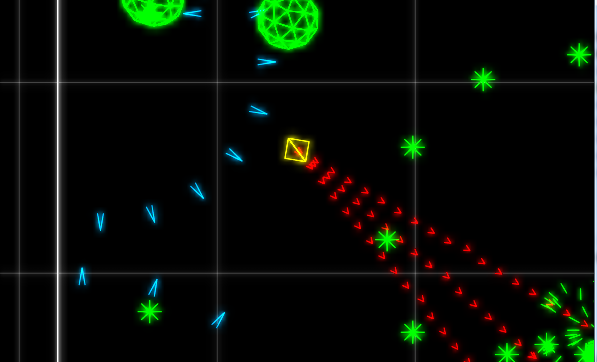
\includegraphics[width=0.7\textwidth]{screenshot1_crop.png}
\caption{In-Game Screenshot}
\end{figure}

Es gibt zwei unterschiedliche Arten von Gegnern: \textit{Seeker} und \textit{Bomber}. Seeker sind sehr klein und lassen sich mit einem einzigen Schuss zerstören, dafür sind sie schnell und treten in Schwärmen auf. Bomber sind schwerfällig, groß und halten mehrere Salven aus. Wenn ein Bomber zerstört wird wird ein Fächer von mehreren Bomben abgeschossen, die nicht abgeschossen werden können. Ziel des Spiels ist es, mit keinem Gegner zu kollidieren und dabei soviele Gegner wie möglich auszuschalten. Der Prototyp ist in dieser Hinsicht allerdings nur bedingt voll ausgebaut, da das eigene Schiff aktuell keine Lebensenergie besitzt und deshalb nicht vernichtet werden kann. Effektiv ist es also unmöglich zu verlieren.

\begin{figure}[H]
\centering
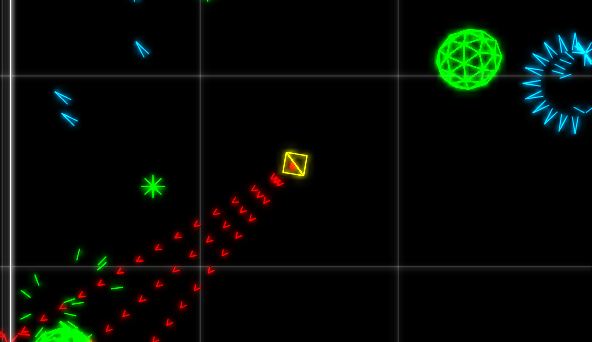
\includegraphics[width=0.7\textwidth]{screenshot2_crop.png}
\caption{In-Game Screenshot}
\end{figure}

\newpage
\section{Implementierung}
Der Prototyp wurde auf Basis der jVR-Rendering-Engine entwickelt und, mit Ausnahme der Shader-Programme, komplett in Scala geschrieben.

\subsection{Architektur}
Die grundlegende Architektur orientiert sich am Actor-Modell von Scala bei dem unterschiedliche Komponenten eines Systems mithilfe von \textit{Messages} kommunizieren. Diese Messages oder auch Events sind einfache Case-Klassen wie in Listing. \ref{caseclass} zu sehen. 

\begin{listing}[H]
\inputminted[firstline=6, lastline=9]{scala}{../scala/org/whiskeysierra/powpow/Messages.scala}
\caption{Message Case-Klassen}
\label{caseclass}
\end{listing}

Die eigentliche Idee des klassischen Actor-Modells ist es, robuste nebenläufige Programme zu schreiben, die weniger anfällig für Fehler sind. In diesem Prototypen wird komplett singlethreaded gearbeitet und Actors kommunizieren synchron. Weiterhin werden Messages nicht direkt an einen bestimmten Adressaten weitergereicht sondern mithilfe eines Broadcast-Mechanismus im gesamten System verteilt. Abbildung \ref{architecture} skizziert den schemenhaften Aufbau des Systems. 

\begin{figure}[H]
\centering
\circledigraph[height=0.75\textwidth]{events} {
    ranksep=2.5;
    edge [dir="both"]
    Displayer -> MessageHub
    Space -> MessageHub
    Grid -> MessageHub
    Ship -> MessageHub
    Camera -> MessageHub
    Gun -> MessageHub
    Swarm -> MessageHub
    Squadron -> MessageHub
    Particles -> MessageHub
    Bombs -> MessageHub
    Keyboard -> MessageHub
    GameController -> MessageHub
}
\caption{Event-based architecture}
\label{architecture}
\end{figure}

\newpage
Alle Subsysteme kommunizieren ausschließlich mit dem zentralen \textit{MessageHub}, der dann wiederum eingehende Nachrichten alle alle anderen Komponenten übermitteln. Das sorgt für sehr entkoppelte Teile der Software, die komplett unabhängig modifiziert oder komplett ersetzt werden können. So ist es beispielsweise unerheblich ob der Spieler die Tastatur oder einen Game-Controller zum Spielen benutzt, solange sowohl die \textit{Keyboard}- als auch die \textit{GameController}-Klasse die gleichen Messages benutzen, müssen alle anderen Teile der Software nicht verändert werden. Zusätzlich lässt sich das verteilte Abarbeiten bestimmter Ereignisse so besser auf bestimmte Klassen verteilen. So gibt es beispielsweise das Event \textit{BomberCollision} das benutzt wird, wenn der Spieler einen \textit{Bomber} rammt. Wenn das passiert sollen einerseits Partikel ausgeschüttet, um den Zusammenprall zu visualisieren, als auch der GameController mit Force Feedback zum Vibrieren gebracht werden. Beide Aktionen sind Folgeaktionen des gleichen Ereignisses aber so grundverschieden, dass sie in verschiedenen Klassen implementiert werden sollten.

Die Implementierung des \textit{MessageHub}s ist dank Scalas Pattern Matching und Closures denkbar einfach wie in Abbildung \ref{messagehub} zu sehen ist.

\begin{listing}[H]
\inputminted[firstline=3]{scala}{../scala/org/whiskeysierra/powpow/MessageHub.scala}
\caption{MessageHub}
\label{messagehub}
\end{listing}

\subsection{jBullet}
Die komplette Physik im Prototypen wird mithilfe von JBullet, dem inoffiziellen Java-Port der Bulletphysics Engine, berechnet. Dazu beerbt jede Klasse, die als Teil der virtuellen Welt in die Physikberechnung einwirken soll, den Trait \textit{Physical}. Viele jBullet-spezifische Konvertierungen und Umrechnungen finden hier statt. Abbildung \ref{physical} zeigt anhand des \textit{position}-Members wie diese Umrechnungen zwischen \textit{jBullet}- und \textit{jVR}/\textit{javax.vecmath}-Klassen hinter einer einfachen API abstrahiert werden können.

\begin{listing}[H]
\inputminted[firstline=25, lastline=34]{scala}{../scala/org/whiskeysierra/powpow/Physical.scala}
\caption{Physical}
\label{physical}
\end{listing}

\subsection{Geometry Shader und Partikelsysteme}
Im Prototypen kommen fünf verschiedene Geometry Shader-Programme zum Einsatz wobei vier jeweils für ein bestimmtes Partikelsystem zuständig sind. Die Geometry Shader werden effektiv benutzt um jegliche Geometry, die im Prototypen vorkommt, zu rendern mit Ausnahme des Schiffes und der \textit{Bomber}, die mithilfe zweier Collada-Modelle realisiert wurden. Alle Partikelsysteme werden durch einen einzigen Knoten im Szenengraph repräsentiert der die gesamte Verwaltung aller Partikel übernimmt. Dazu zählen der gesamte Lebenszyklus einzelner Instanzen, das Wiederverwenden/Recyclen, die Konfiguration und Integration des zugehörigen Geometry Shaders sowie die Interaktion mit dem restlichen System mithilfe des Message-Systems.

Abbildung \ref{scenegraph} zeigt einen Ausschnitt des Szenengraphen mit allen Knoten, die ihre Geometry mithilfe eines Shaders generieren, ein Partikelsystem verwalten oder beides.

\begin{figure}[H]
\centering
\digraph[height=\textwidth]{scenegraph} {
    ranksep=2.5;
    Root -> Bombs
    Bombs -> Bomb [label="1:*"]
    Root -> Gun
    Gun -> Bullet [label="1:*"]
    Root -> Grid
    Root -> Particles
    Particles -> Particle [label="1:*"]
    Root -> Swarm
    Swarm -> Seeker [label="1:*"]
    Root -> Squadron
    Squadron -> Bomber [label="1:*"]
}
\caption{Szenengraph}
\label{scenegraph}
\end{figure}

\subsection{Postprocessing und Wireframes}
Einen Großteil des visuellen Eindrucks des Prototypen wird durch zwei wichtige Effekte hervorgerufen: Wireframe-Darstellung und der Glow-Effekt. Der Wireframe-Effekt wird mithilfe der OpenGL-Funktion \textit{glPolygonMode} realisiert wie Listing \ref{wireframe} zeigt. Dabei werden Polygone nicht mehr als ausgefüllte Dreiecke gerendert, sondern nur deren Ränder.

\begin{listing}[H]
\inputminted[firstline=10, lastline=10]{scala}{../scala/org/whiskeysierra/powpow/EnableWireframe.scala}
\caption{OpenGL Wireframe Mode}
\label{wireframe}
\end{listing}

Der Glow-Effekt ist als \textit{Bloom}-Shader mit Multipass-Rendering implementiert. Dazu wird die Geometry in einem ersten Durchgang in ein \textit{FrameBufferObject} gerendert, auf das dann wiederum in einem zweiten Durchgang als Textur zugegriffen werden kann. Dazu wird ein einfaches Quad mithilfe eines Fragment-Shaders gerendert.

\begin{listing}[H]
\inputminted[firstline=34, lastline=53]{scala}{../scala/org/whiskeysierra/powpow/PowPow.scala}
\caption{Multipass Rendering}
\label{multipass}
\end{listing}

Das Rendern des \textit{FrameBufferObject}s auf ein Quad mithilfe eines Fragment-Shaders funktioniert natürlich im Wireframe-Modus nur bedingt da einzig die Kanten sowie eine Diagonale gerendert werden. Um diesen Umstand zu umgehen muss in der Pipeline festgelegt werden, dass vor dem Rendern der eigentlichen Geometry der Wireframe-Modus aktiviert und vor dem zweiten Durchgang wieder deaktiviert wird. Die \textit{Pipeline}-Klasse des jVR-Frameworks bietet leider keine öffentliche API an die es erlauben würde selbstgeschriebene \textit{PipelineCommand}s zu registrieren. Als Workaround wurde in diesem Prototypen via Reflection auf die private Methode \texttt{Pipeline.addCommand(PipelineCommand)} zugegriffen wie in Listing \ref{multipass} zu sehen ist.

\newpage
\nocite{pewpewgame}
\nocite{jinput}
\nocite{scala}
\nocite{jbullet}
\nocite{BaileyCunningham200905}
\addcontentsline{toc}{section}{Literatur}
\printbibliography

\addcontentsline{toc}{section}{Abbildungsverzeichnis}
\listoffigures

\addcontentsline{toc}{section}{Quellcodeverzeichnis}
\renewcommand\listoflistingscaption{Quellcodeverzeichnis}
\listoflistings

\end{document}

